\documentclass[pdftex,12pt,a4paper]{article}
\usepackage{amsthm}
\usepackage{amssymb}
\usepackage{enumerate}
\usepackage{amsmath}
\usepackage{verbatim}
\usepackage{graphicx}
\usepackage{hyperref}
\usepackage{fancyhdr}

\newcommand{\HRule}{\rule{\linewidth}{0.5mm}}


\pagestyle{fancy}

\fancyhead[RO,RE]{Peter Zhang and Carl Jackson}
\fancyhead[LO, RE]{CS 171: Project 3}

\begin{document}
\begin{titlepage}
\begin{center}

% Upper part of the page. The '~' is needed because \\
% only works if a paragraph has started.

\includegraphics[width=0.15\textwidth]{twitterlogo.jpg}~\\[1cm]


\textsc{\Large CS 171: Project 2}\\[0.5cm]

% Title
\HRule \\[0.4cm]
{ \LARGE \bfseries Pheme: \\ Birds of a Feather Tweet Together} \\[0.4cm]

\HRule \\[1.5cm]

% Author and supervisor
\begin{minipage}{0.6\textwidth}
\begin{flushleft} \large
\emph{Authors:}\\
Carl Jackson and Peter Zhang
\end{flushleft}
\end{minipage}
\begin{minipage}{0.4\textwidth}
\begin{flushright} \large
\end{flushright}
\end{minipage}

\vfill

% Bottom of the page
{\large \today}

\end{center}
\end{titlepage}
\tableofcontents
\pagebreak

\section{Introduction}
\subsection{Motivation}
Most current visualizations of social data require viewers to already have a subject matter in mind; they allow viewers to search for and investigate specific keywords, hashtags, or locales. However, we think that social data is interesting primarily because it allows us to discover new topics for investigation - topics that are being generated in real time by the humans who are producing the social data. Accordingly, we want to build a visualization that guides a curious but unfocused viewer in identifying undiscovered topics/events that are currently occurring in the real world. Furthermore, we hope to help users learn about and experience these events through the social data they generate. In this way, we hope that our visualization not only tells a story, but tells a unique story to every viewer, depending on what they are interested in and when they are accessing our visualization. 


\subsection{Goals}
The two overarching research questions of our visualization for projects II and III are:
\begin{enumerate}
\item Can we identify "events" from real-time social data?
\item If we can, what can we learn about such "events"?
\end{enumerate}
In project II, we built a visualization that tries to identify current events that are occurring in a user-specified geography (location + radius), using real time social data. Concretely, we pull a live stream of Twitter data arriving from the specified geography, and try to identify clusters of tweets; we were clustering primarily by geographical proximity. In effect, we've covered question $1$ from above in Project II.

In project III, we have achieved two goals in addition to event identification. First, we've worked on improving our visualization from Project II to allow users to not only identify current events, but help them learn and experience the events that they have identified. In Pheme 2.0, we've performed some basic natural language processing - word frequency analysis - and visualized this analysis to help users identify the nature and context of the event they have identified. Additionally, we allow users to explore the data within an event temporally, seeing the frequency of tweets over time and filtering events by time range. Second, we've built a significantly more involved server-side component to our visualization, which is constantly identifying events all over the world from live tweet data. Accordingly, users now have two choices for visualizing events; they can either use the live-streaming mode to identify events in real time and then learn about them, or explore pre-recorded events in more depth using the advanced visualization techniques mentioned above in Pheme 2.0. Finally, we also significantly improved the event identification process that we had developed in Project II; the events that we now identify are significantly higher quality. 

\section{Description of Data}
\subsection{Source}
As in Project II, the ultimate source of the data for our visualizations is Twitter, an online social network and microblogging service that allows users to instantaneously send and receive short messages, called tweets, on various electronic devices. Twitter is one of the most popular, if not the most popular, sites that produces real-time social data; as of 2012, it produced more than 340 million tweets per day \footnote{http://techcrunch.com/2012/07/30/analyst-twitter-passed-500m-users-in-june-2012-140m-of-them-in-us-jakarta-biggest-tweeting-city/}. Given our interest in high-throughput social data streams, Twitter was a natural data source to focus on.

Using Twitter's API, we pulled tweets, which contained several relevant pieces of information:
\begin{enumerate}
\item Geographical location: Twitter users can choose to specify a geographical location to associate with their tweet. This is particularly interesting for users who tweet on their mobile phones, and choose to expose their phone's GPS data to the service.
\item Twitter Screenname: Tweets are associated with the screen name of the user publishing the tweets.
\item Tweet contents: The actual text content of the tweet. This is also available to viewers of our visualization.
\item Hashtags: Twitter users can specify hashtags, or metadata, to associate with their tweet. 
\item Tweet timestamp: The time at which the tweet was published.
\end{enumerate}

\subsection{Scraping Method}

Typically, Twitter's API allows you to view historical tweets, at most a few
hundred at a time, using its REST API. Since we wanted to see tweets as they
happened, we instead chose to rely on Twitter's streaming API, which is a
mechanism by which you can express interest in a particular Twitter search
query, and receive push updates from Twitter as new Tweets are written that
match the query. This live stream is sometimes referred to as the ``Twitter
Firehose,'' although Twitter only makes a subsampling of the full Firehose
available for third party developers.

Twitter's streaming API allows you to search for tweets by geographical
location, so we established a connection to Twitter that requested the Tweets
that would be visible on the user's screen. Each user needed to have their
tweets scraped from a different live API feed, since different users can be
visualizing different portions of the map at once.

One particular challenge involved with Twitter's streaming feed was that of
authentication. Twitter protects their streaming API using OAuth, which is a
mechanism for authenticating individual Twitter users with third party
applications. In order to get access to a live stream of tweets, we must prove
to Twitter that we are doing it on behalf of a valid Twitter user, and obtaining
these credentials is a particularly finicky multi-step process. Only after
forcing users to authenticate can we proceed with our visualization.

\section{Related Work}
To the extent that we've used what we've learned so far in CS 171, all the readings and lecture materials are related work; when justifying our visualization choices or visualization evolution, we will refer to this material. We consulted documentation related to the Twitter API and the Google Maps API very often while working on this project. In addition, we were inspired to investigate and study tweets and their geographical data by a past CS 171 project: Tweetography. \\ \\
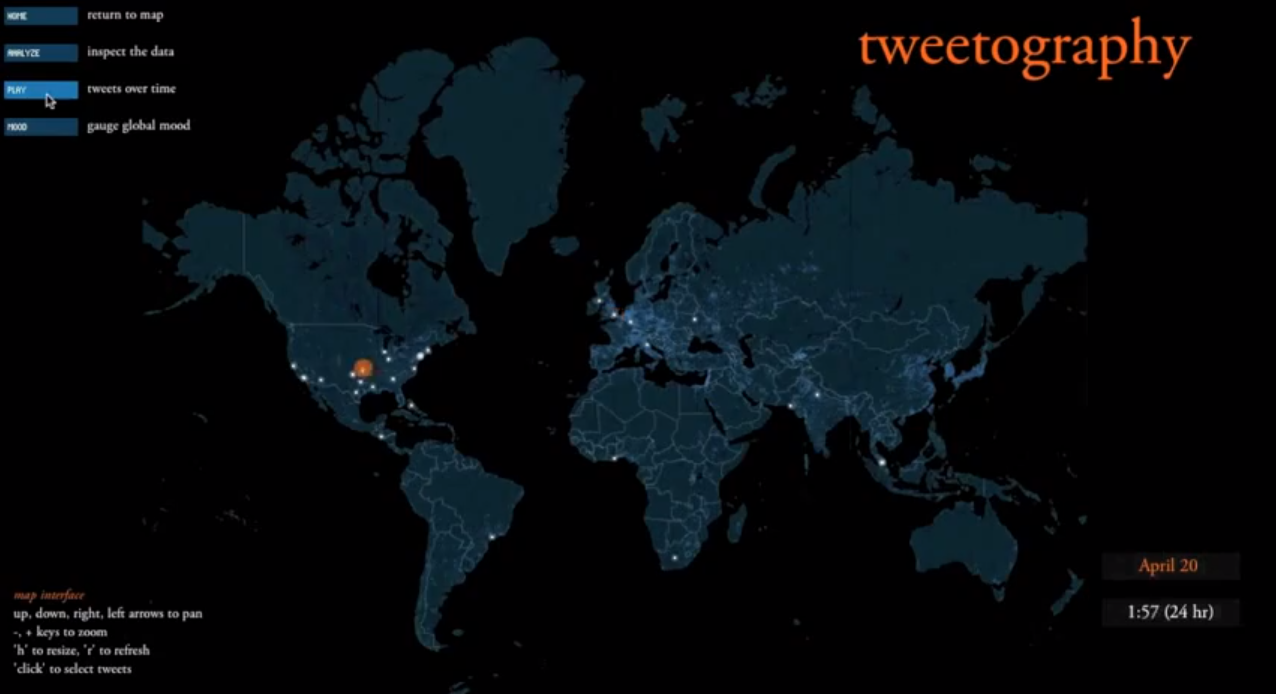
\includegraphics[width=5.5in]{tweetography.png} \\ \\
We found the concept of tweets appearing over time on a map very attractive, and based our visualization on this concept, even though the purpose and design of our visualization is very different than Tweetography.
In addition to this source of inspiration for our overall visualization, there are several other sources which have guided us in specific design choices we've made (discussed in design evolution below):
\begin{enumerate}
\item In designing our tweet content visualization, which required some very basic natural language processing, we referred to several sources. \\ http://www.wordle.net/ and http://www.jasondavies.com/wordcloud/ gave us guidance on how to design word clouds, although our final design was markedly different. We referred to http://norm.al/2009/04/14/list-of-english-stop-words/ in deciding how to process the text of tweets.
\item In designing the temporal aspect of our visualization - which allows users to explore the tweet data in an event by time - we were inspired by http://bl.ocks.org/mbostock/1667367; using this framework, we built a tweet frequency over time chart that was linked to our main visualization via brushing. 
\end{enumerate}

\section{Design Evolution}
At the end of project II our visualization was basically just tweets placed on a map, a sidebar containing a list of clusters and the tweets within the clusters, and a visual representation of the clusters on the map. A screenshot of our progress at that point can be found below: \\ \\
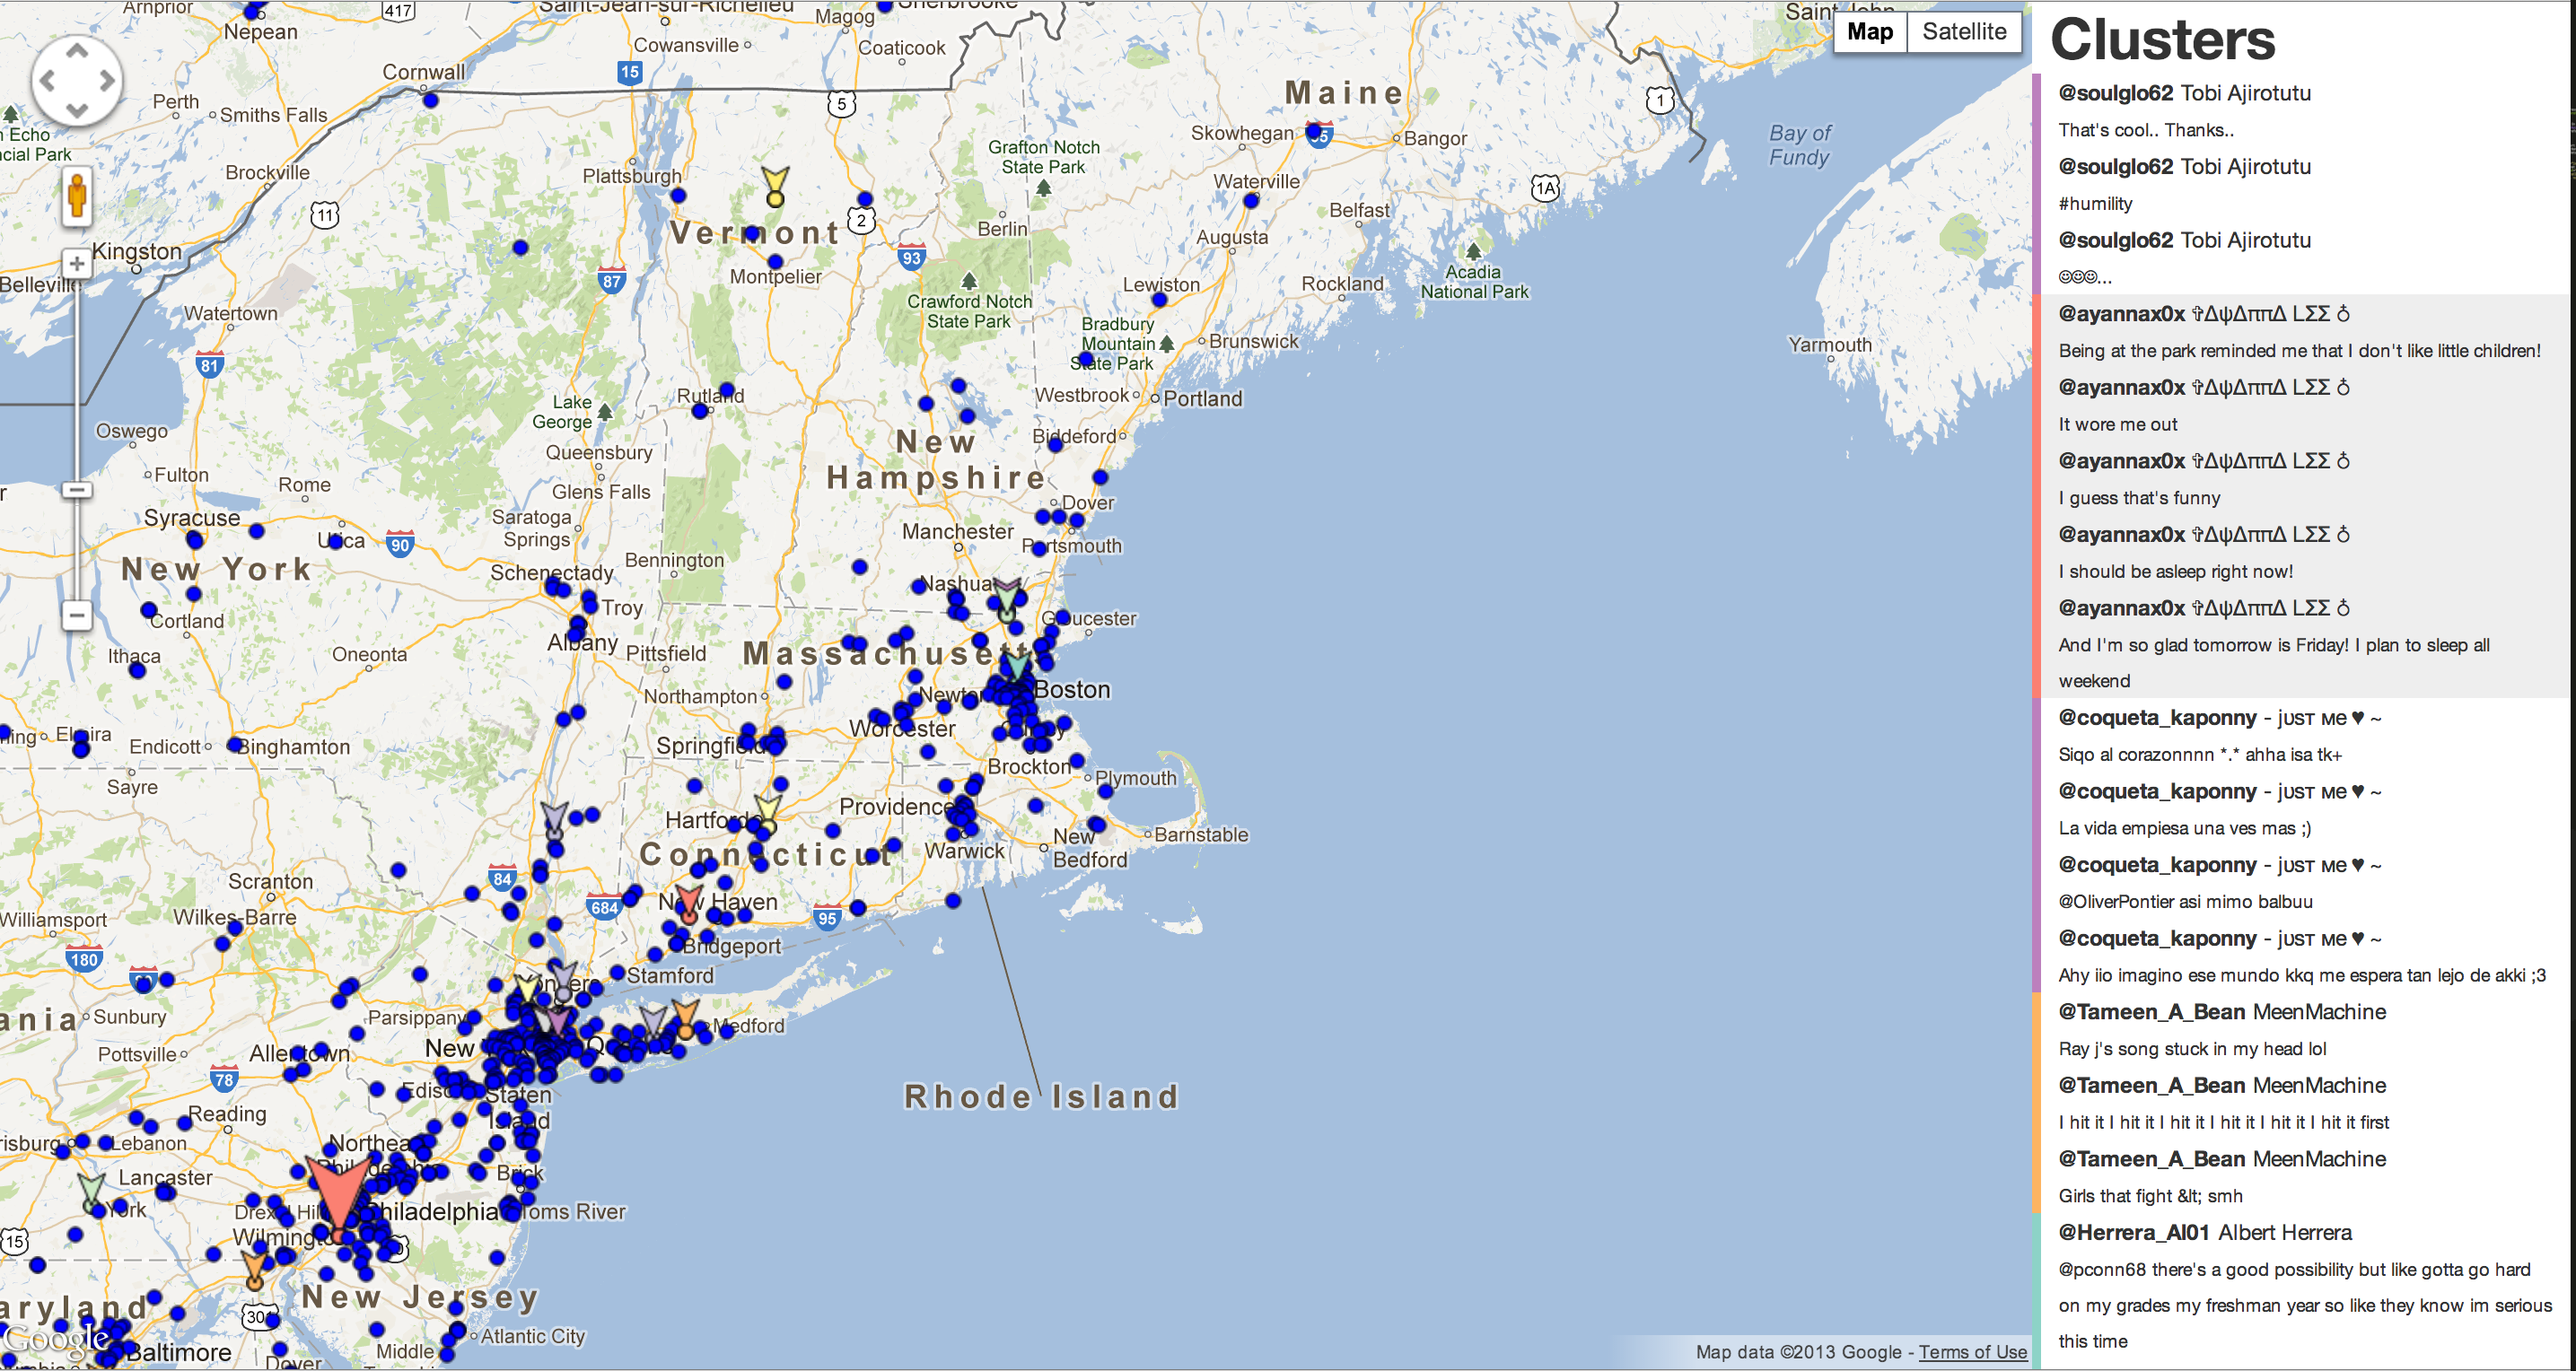
\includegraphics[width=5.5in]{project2.png} \\ \\
Coming into project III, we had several specific issues that we wished to address about project II, as well as several specific goals (some of which address the issues mentioned) for project III:
\begin{enumerate}
\item Issues:
\begin{enumerate}
\item The visualization was somewhat confusing without the process book.
\item The visualization became slow and cluttered as more and more tweets arrived.
\item Some identified clusters were low quality (did not correspond to real events).
\item Tweets arrived slowly at certain locales at certain times of day.
\end{enumerate}
\item Goals:
\begin{enumerate}
\item Help users learn about the subject matter of an event.
\item Help users explore an event temporally.
\item Let users explore pre-recorded events. 
\end{enumerate}
\end{enumerate}
These issues and goals presented both significant technical and visualization design challenges. We discuss the evolution of our attempts to address them in the two subsections below. Specifically, we  address 1(a), 1(d), and 2(c) in 4.2.1, 2(a) in 4.2.2, 1(b) in 4.2.3, 1(c) in 4.2.4, and 2(b) in 4.2.5.

\subsection{Technical Design}

\subsection{Visualization Evolution}
\subsubsection{User Flow}
One of the biggest problems with our project II was that it was confusing to new users who did not have access to our process book. To address this issue, we decided to make a splash page explaining the key parts of our visualization, as shown below: \\ \\
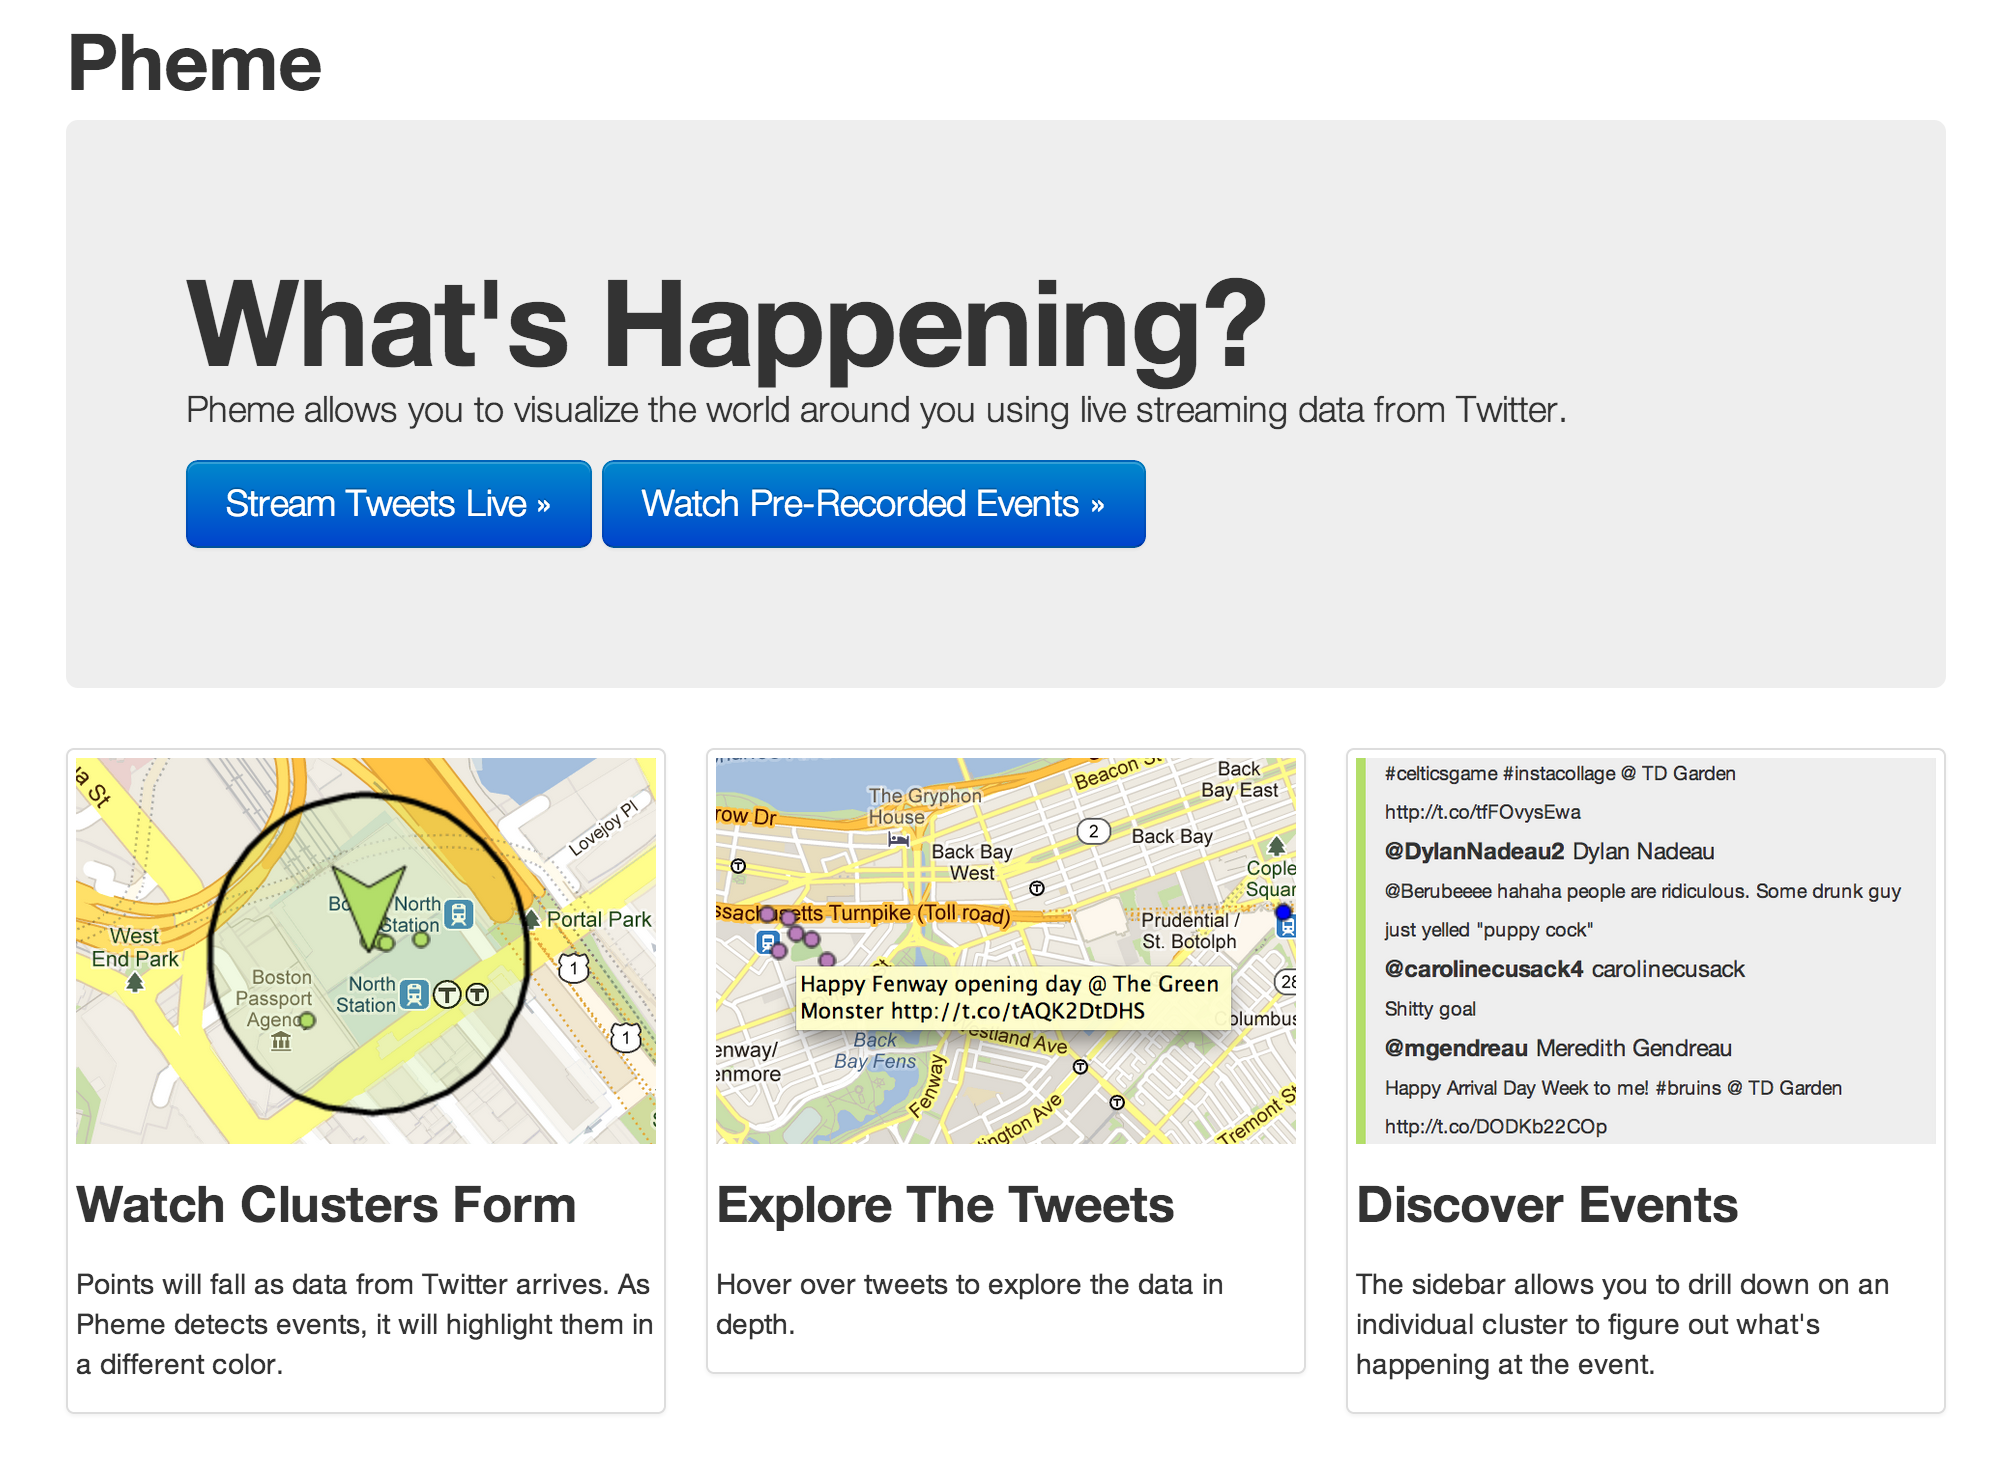
\includegraphics[width=5.5in]{splash.png} \\ \\
In this way, we strengthen the narrative of our visualization; while our visualization does not tell a specific story (since it allows users to discover interesting stories in the world), it does this with specific progression. It \emph{opens} by loading tweets and identifying clusters; users watch as clusters form on the map. The \emph{middle} of this progression allows users to inspect individual tweets on the map by hovering over them, allowing them to understand the social data being produced in and around clusters as the clusters are identified. The \emph{closing} of our visualization allows users to learn about and explore the clusters that have been identified and the events that they represent.

In addition, one of our major goals in Project III was to allow users explore pre-recorded events. This helps address one of the issues we experienced in project II; there was often insufficient live streaming twitter data in a particular locale and at a particular time (because we only get a subsample of the full Twitter firehose), and thus tweets arrived slowly. Now, our visualization is compelling to users even in such a situation, because they can use the visualization to explore events that have been pre-recorded when live data is too sparse. By clicking on the ``Watch Pre-Recorded Events" button on the page shown above, the user is brought to the following page: \\ \\
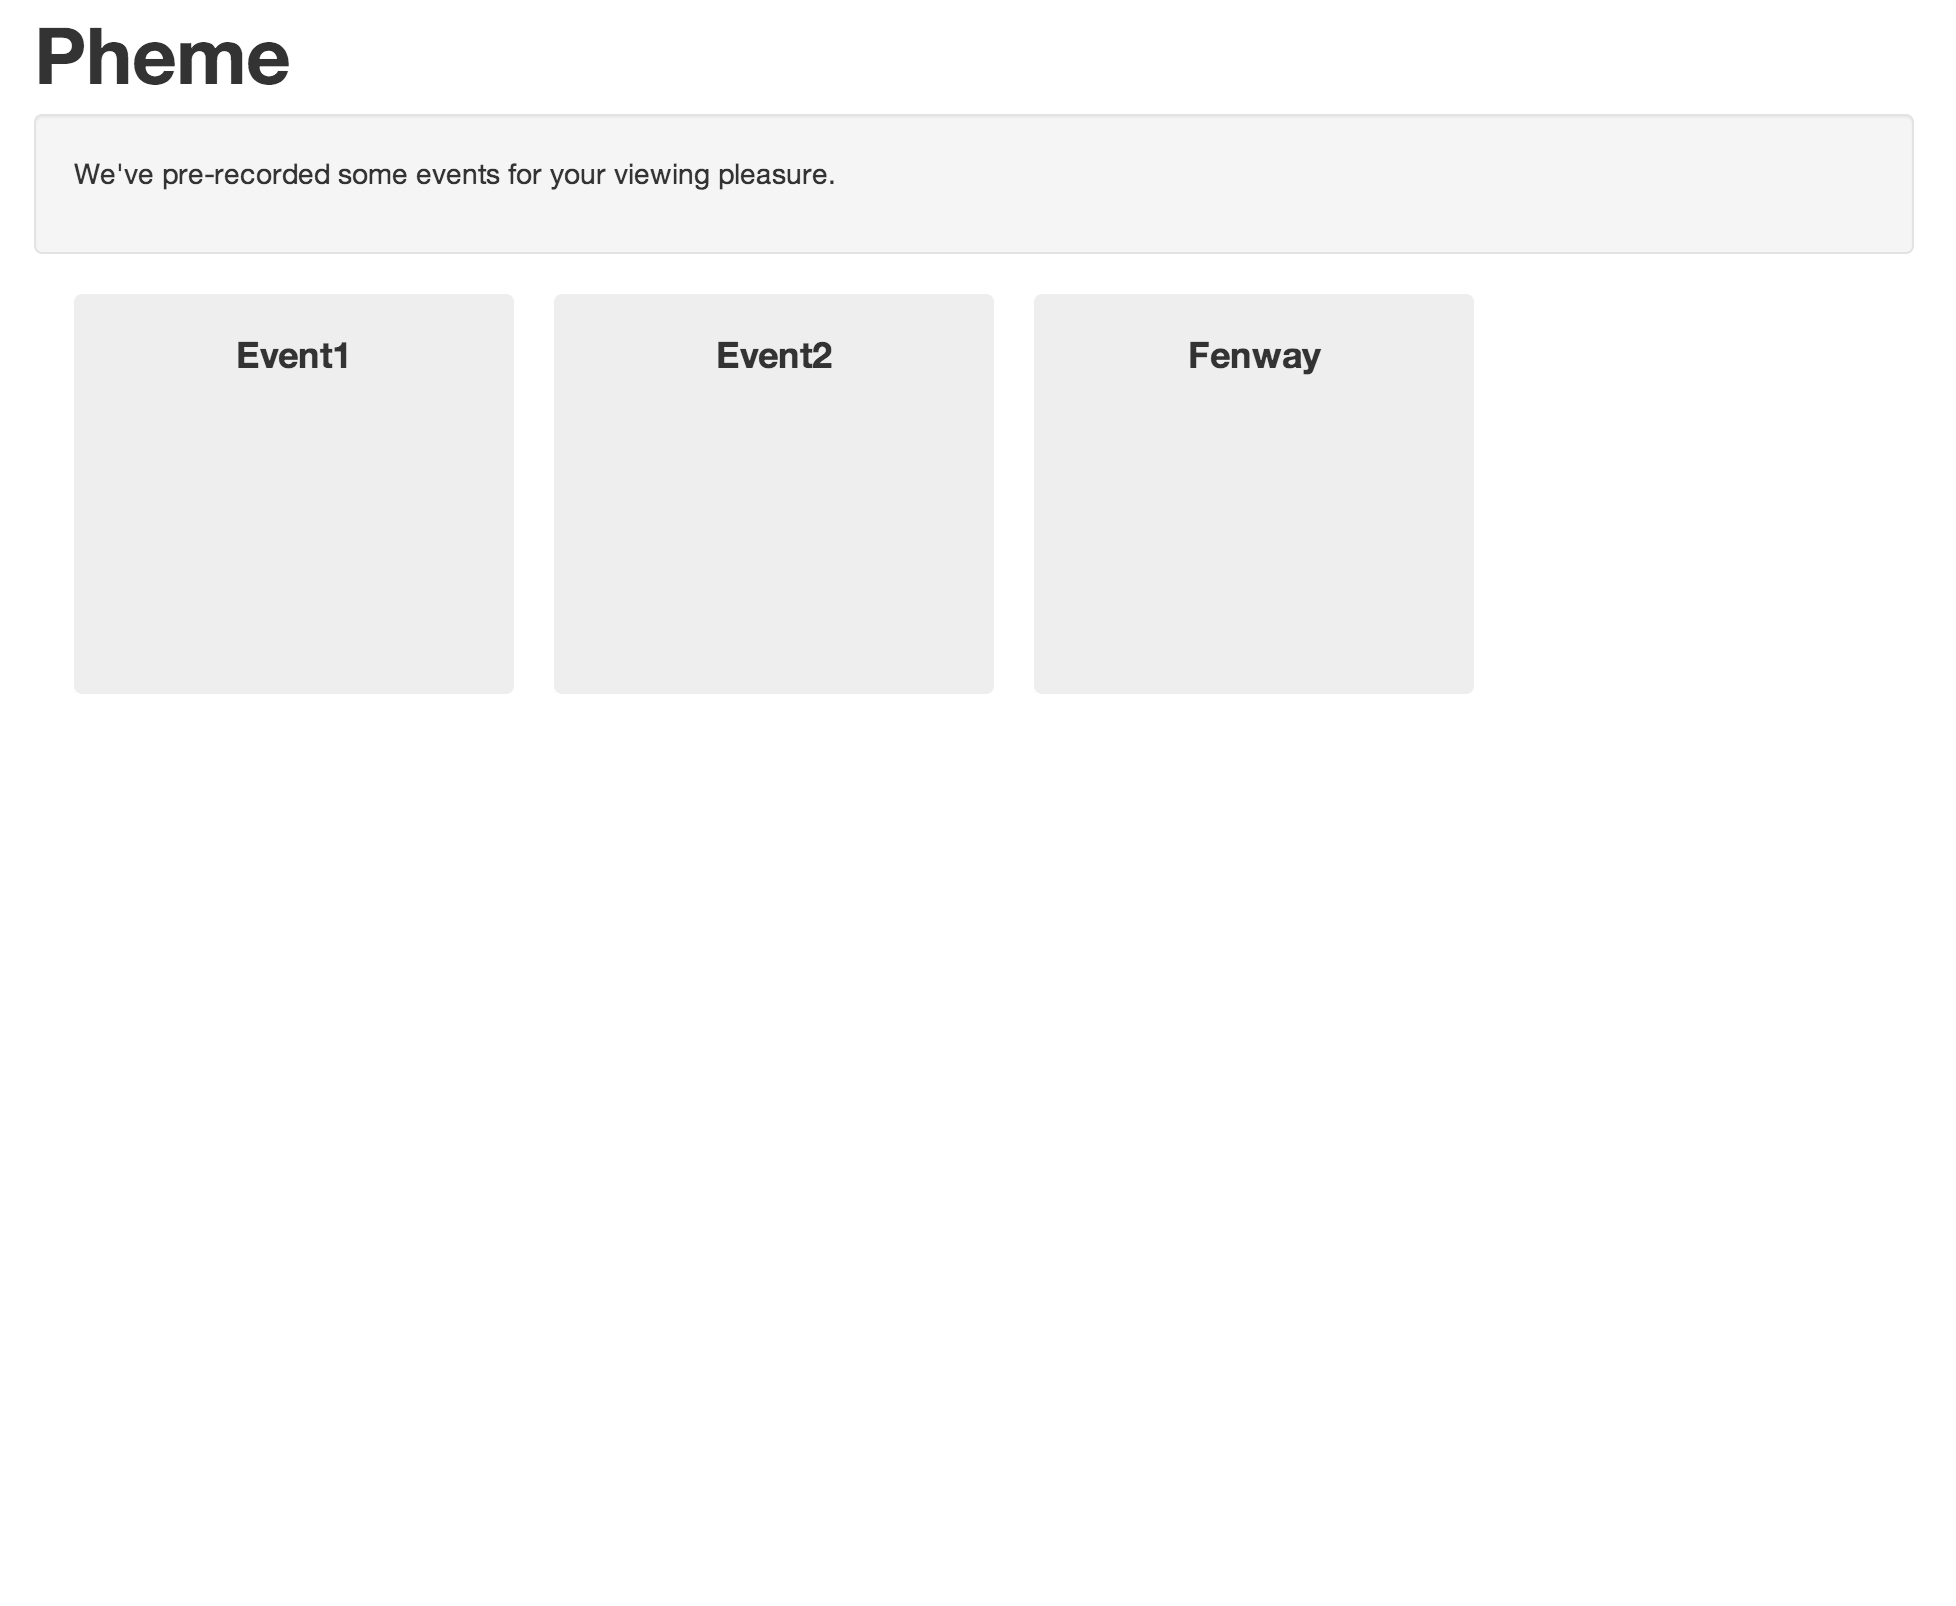
\includegraphics[width=5.5in]{splash2.png} \\ \\
which displays a list of pre-recorded events that they can view in our visualization. 

\subsubsection{Natural Language Processing}
To allow users to learn more about the subject matter of an event, we proposed a complicated visualization that would use several techniques to analyze and visualize this content: \\ \\
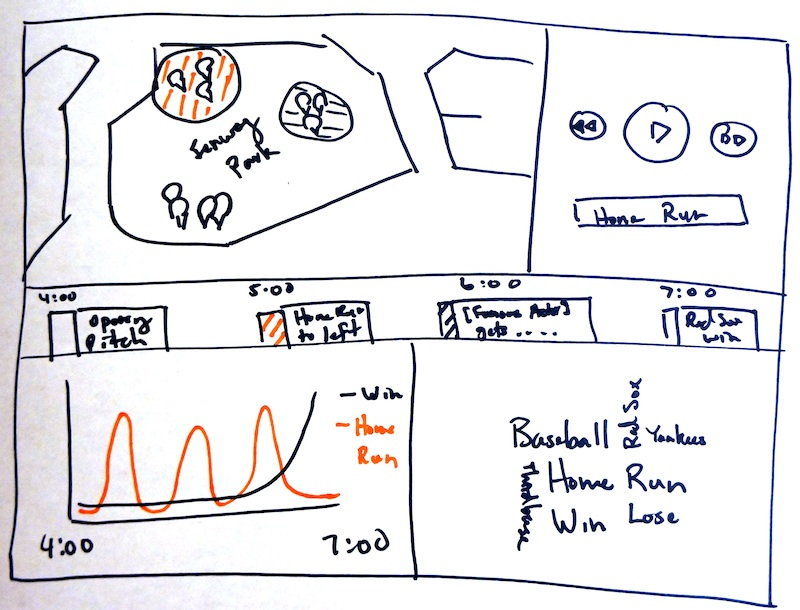
\includegraphics[width=5.5in]{pheme2.jpg} \\ \\
We first decided to attempt to make the word cloud aspect of this proposed visualization. We initially used the http://www.jasondavies.com/wordcloud/ package for generating word clouds. Our first iteration was filled with common english words that provided no significant content, like ``the," ``are" etc. Accordingly, after doing some research, we realized that one of the most common steps in processing natural language is to first filter out what is known as ``stop words" - common words in the english language that crowd out the interesting frequency data; we took a list of ``stop words" from  http://norm.al/2009/04/14/list-of-english-stop-words/. After this filtration, we arrived at a word cloud similar to the following for all the tweet data on the screen: \\ \\
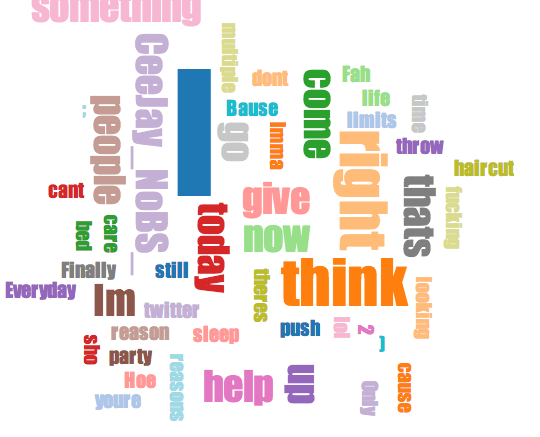
\includegraphics[width=5.5in]{cloud1.png} \\ \\
After some thought, we decided that this was not particularly helpful for viewers, for several reasons. First, the cloud only provided aggregate data about all tweets on screen; however, we were interested in the content of specific clusters. Second, while the bright colors, rotation of words, and large quantity of words were certainly visually attractive, it made it very hard for the viewer to perform any useful visual query on the cloud. Finally, if we put a standalone word cloud on the map, the most important part of our visualization - the map - became uncomfortably small.

Accordingly, we decided on a different use for the word cloud. First, we reduced the number of words in each word cloud to only $10$, so that users would only be presented with the most important words, and be able to quickly enumerate through them. Second, we changed the presentation of the word cloud. Rather than have words rotated at some multiple of $90$ degrees, we instead presented all words in the same orientation, one after the other, so that users could actually read all the words in the word cloud. Furthermore, we encoded the frequency of the word with a dual encoding, using both color and font size, as Tufte suggests. The color we used for each word cloud corresponds to the color we labeled each cluster with; we applied a gradient going from the color of the cluster to grey, so that more important/frequent words were not only bigger, but more colorful. Finally, we used these word clouds as labels for the clusters in the sidebar of our visualization by generating one for each cluster. By combining the sidebar in our original visualization with this new word cloud example, we not only save space and help the viewer associate the textual content of a cluster with the tweets within that cluster (since both are now contained in the sidebar), but also address our original concern that word clouds should provide data about the content of individual clusters rather than aggregate data about all the tweets on the map. We did all this by writing our own simple implementation of a word cloud, rather than using an third-party library. 

We know that word clouds are often frowned upon \footnote{http://www.niemanlab.org/2011/10/word-clouds-considered-harmful/}, but we've attempted to address many of the issues raised about word clouds (by removing extraneous words, increasing the viewer's ability to perform visual queries on data, and removing chart junk like extraneous color); we believe the final result is both effective at visualizing the textual information contained in a cluster of tweets, and still visually attractive. 

\subsubsection{Tweet Fading}
Another problem we experienced in Project II was that our visualization became both slow and difficult to read as more tweets came in. For example, after only a few minutes at a relatively high zoom, our visualization would look like the following: \\ \\
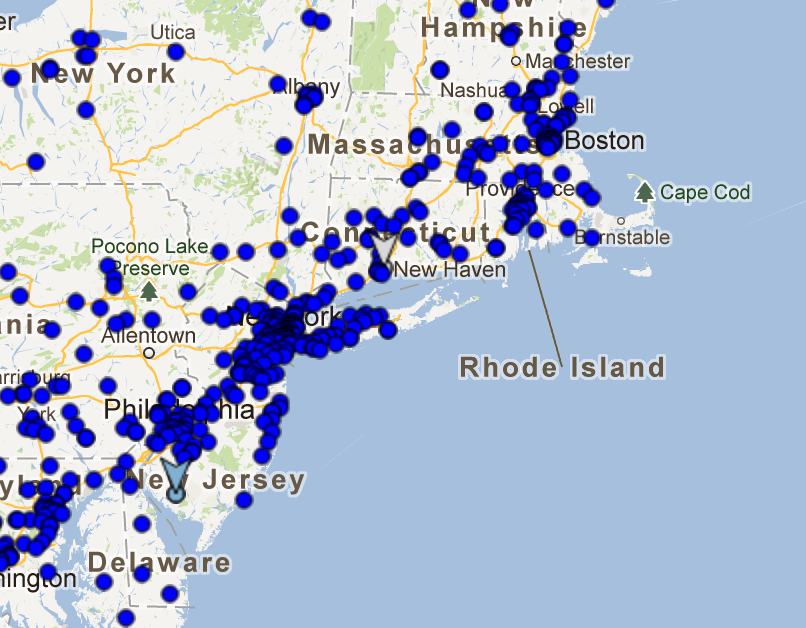
\includegraphics[width=5.5in]{toomuch.png} \\ \\
As shown above, the tweet density rapidly became very high in certain regions, making it hard to read individual tweets, and slowing down the underlying google maps visualization. To address this problem, we suggested a simple solution: fade out old tweets. We envisioned the process would look something like the following: \\ \\
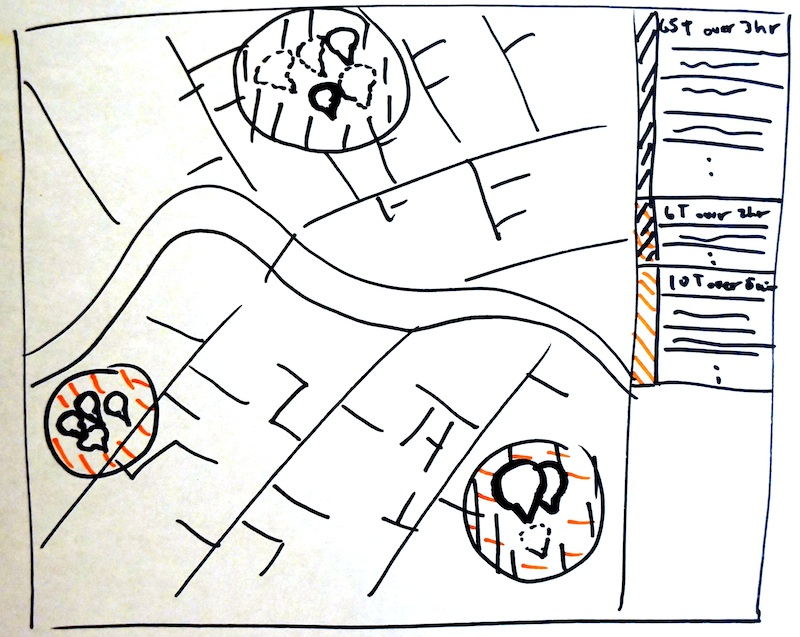
\includegraphics[width=5.5in]{pheme4.jpg} \\ \\
Our final implementation is very similar. The opacity of a tweet slowly decreases as time goes on, as shown below: \\ \\
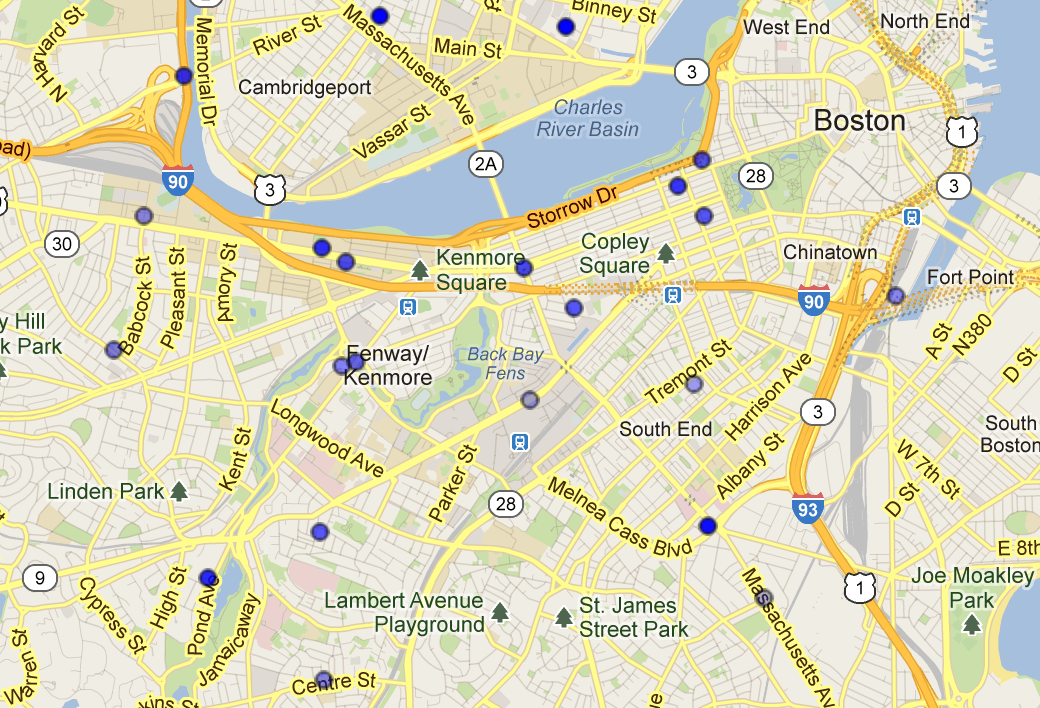
\includegraphics[width=5.5in]{fading.png} \\ \\
Furthermore, if tweets reached a certain age, they would disappear completely; this helps not only reduce clutter, but increase the performance of our visualization. The speed of fading, and the age at which the tweets 

\subsubsection{Clustering Improvements}
In Project II, one of the issues we noticed was a significant percentage of bad clusters. We identified two major reasons why these clusters were occuring. 

First, we noticed that many of our clusters resulted from a single person tweeting multiple times rapidly form the same location. For example, one of the clusters we found in our original visualization was as follows: \\ \\
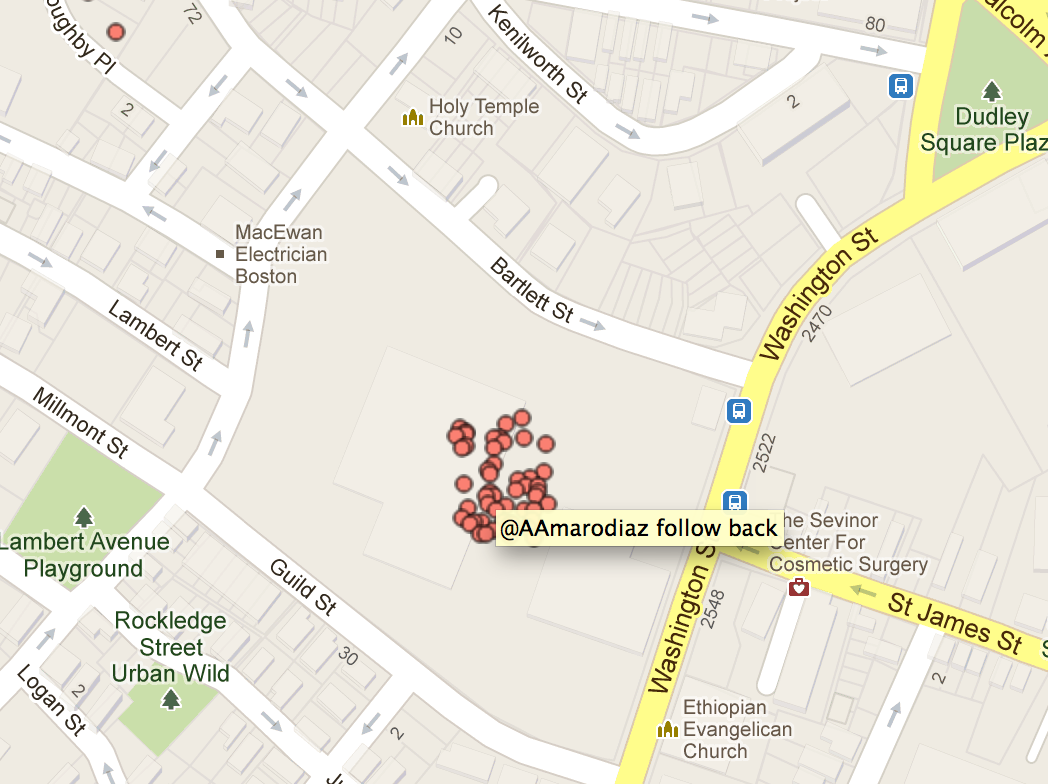
\includegraphics[width=5.5in]{lonely.png} \\ \\
This is a single person tweeting to tens or hundreds of other people asking them to follow him/her. Clearly this type of cluster is not actually an event. Accordingly, we designed several ``quality" checks to make sure that the clusters we identified were actually interesting. In particular we checked if:
\begin{enumerate}
\item $\frac{[\text{\# of authors}]}{[\text{\# of tweets}]} < 40\%$. We made this check because it is likely that the clusters of tweets that are most likely to correspond to real events, rather than several local friends tweeting at each other or a single person tweeting from the same place frequently, are clusters where many different people have tweeted in the same location. Thus, we reject all clusters where there are relatively few authors per tweet, since that implies that the majority of tweets were authored by the same person. 
\item Reject if $[\text{\# of tweets}] < 6$ and no two tweets share at least one word. We made this check because we didn't want to cluster tweets that happened to be geographically close together by chance. Accordingly, if there are only a few tweets in our cluster, we make sure that they are related by checking if they share words; however, if there are large number of tweets in our cluster, it is extremely unlikely they occurred by chance, and thus don't need to make that check.
\end{enumerate}

Second, we noticed that if we let our clustering algorithm run for long periods of time, the clusters we identified would continue to grow larger. This is because our original algorithm adds a new tweet to a cluster when the new tweet is close to \emph{any} of the tweets currently in the cluster. Accordingly, the larger a cluster is, the more likely it is that a new tweet will join to it; there is an unwanted snowball effect. To combat this effect while still maintaining an incremental clustering algorithm (so that our visualization would run at reasonable speeds), we included a temporal aspect to the ``closeness" metric in our clustering algorithm. In particular, when we measure how far away two tweets are, we measure their distance not only geographically, but also temporally. With this new metric, a large cluster isn't quite as likely to snowball in size, since new tweets are only ``close" to tweets in the cluster that are relatively recent. 

\subsubsection{Tweet Scrubber}
One of the major goals we had for Project III was to allow users to explore events that have been identified or pre-recorded temporally. Originally, we had two proposals for doing this. First, we considered a youtube style player, which would allow users to play back, fast forward, and rewind an event, watching tweets fall at normal speed, higher speed, or watching the tweets disappear. We envisioned it as something similar to the following:\\ \\
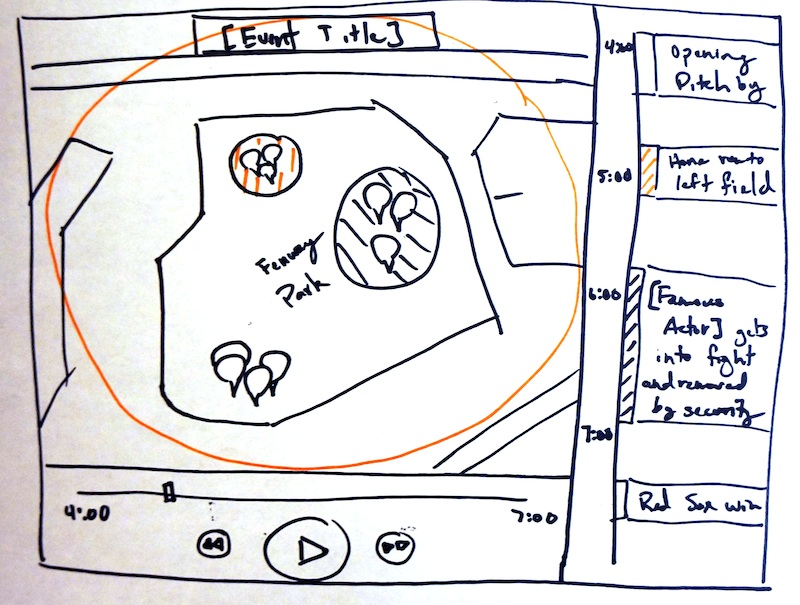
\includegraphics[width=5.5in]{pheme3.jpg} \\ \\
After some more thought, we decided that this wasn't necessarily the right paradigm for temporal exploration of an event; it did not give the user sufficient control over the viewing experience. Instead, we proposed the following: \\ \\
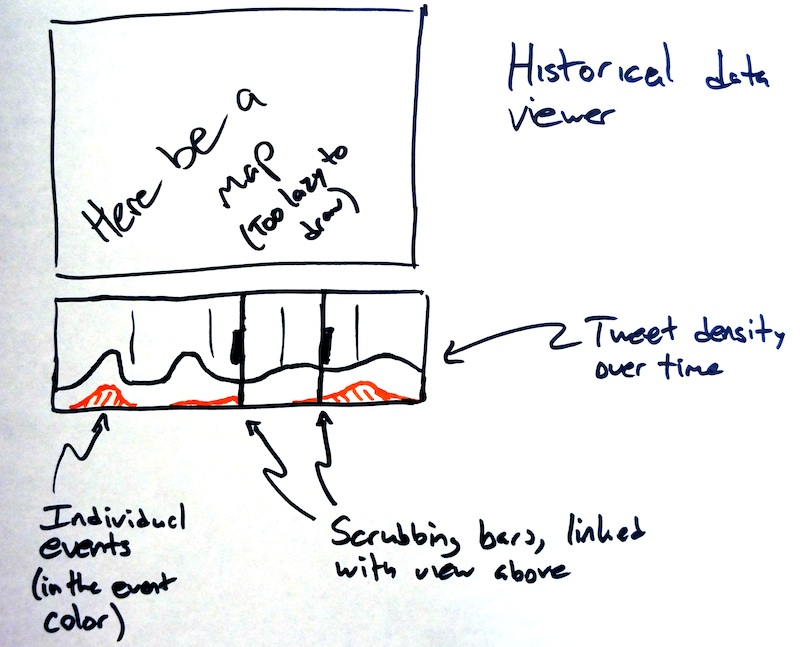
\includegraphics[width=5.5in]{pheme5.jpg} \\ \\
In this proposed visualization, the line chart below the map displays tweet frequency over time (with the x-axis encoding time). Users can brush the line chart by specifying a range of times using two scrubbers, and only tweets that fell during that time range will appear on the map. In this way, users can go through the historical stream of tweets with a fine-toothed comb, temporally, selecting exactly the time range they are interested in and investigating that range. Our final implementation of this feature is relatively similar, as shown below: \\ \\
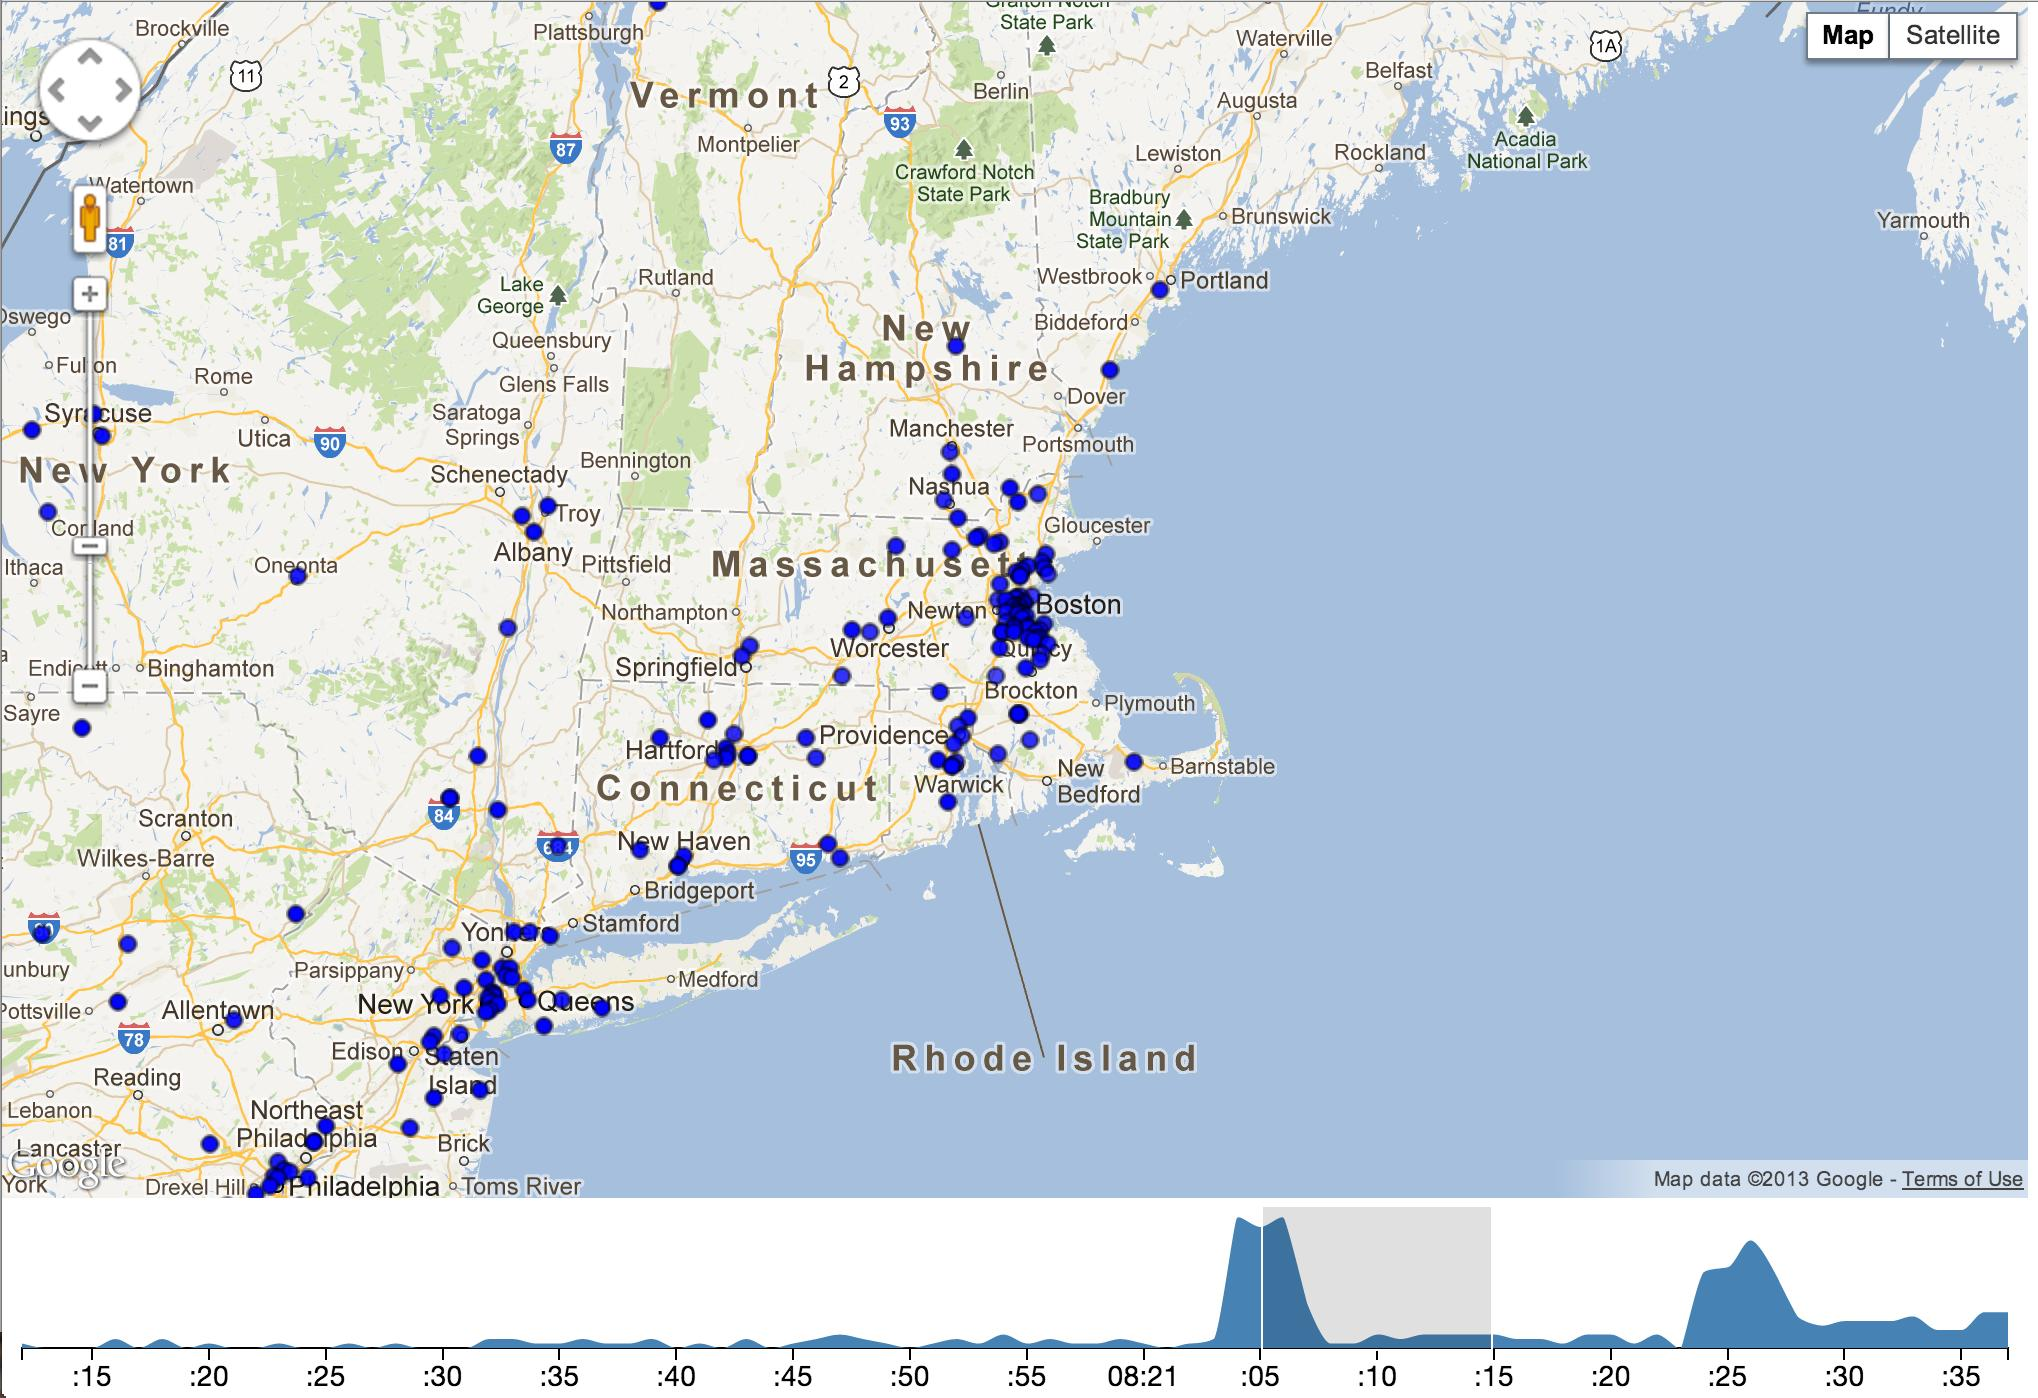
\includegraphics[width=5.5in]{temporal.jpg} \\ \\
Once difference to note is that the line chart no longer displays the tweet frequency of the clusters. This is due to the fact that the temporal tweet density for a cluster is too low, so there is no useful information to be gained there. 

\section{Visualizations and Discussion} 
\subsection{Visualization}
Our visualization allows the user to select a geography of interest, and to draw tweets on the map in real time. By default, our visualization is currently focused on Boston; however, users can zoom and drag the map as desired to grab tweets from any particular region in the world. As data arrives, we also dynamically detect clusters of interesting points in the current viewport/geography, and visually group them by enclosing them in a circle and coloring them similarly. In addition, we display a list of all the identified clusters, the component tweets in each cluster, and a word cloud summarizing the cluster, in a secondary view - a sidebar to the the right of the map. Finally, we have a tertiary view below the map, which is a line chart displaying temporal data about the frequency of tweets over time.Our visualization also supports several user interactions, as described below:
\begin{enumerate}
\item Linking \& Brushing. Our visualization has three views, the map - which displays the geographical location of tweets and clusters - the cluster sidebar - which contains a list of all clusters currently identified, a word cloud summarizing the cluster, the member tweets of each cluster - and the tweet frequency line chart - which displays data about the frequency of tweets arriving over the course of the visualization. We support linking \& brushing by interactively highlighting the cluster marker on the map (by making it larger) when ther viewer hovers over the cluster in the cluster sidebar, as well as brushing a specific section of the line chart to display only tweets that occurred within that time frame.
\item Details-on-Demand. Our visualization supports details-on-demand with a tool tip. Whenever a user hovers over an individual tweet on the map, regardless of whether or not it is in a cluster, a tool tip will appear after a short delay showing the text contained in the tweet. 
\item Drill-Down/Filter Capability. Our visualization suuports a drill-down or filtering interaction by allowing users to drag the map viewport and zoom in or out of the viewport as desired. In this way, the user can exactly specify what geographical area they wish to pull tweets and identify clusters in; the visualization responds by drilling-down/filtering tweets to match this specification. 
\end{enumerate}

\subsection{Discussion}
The primary goal of our visualization is two-fold: to identify events in the world as they were happening, and allow to user to learn and experience these events through the social data they produce. We began work on the first half of our goal in Project II. In Project III, we've both continued working on event identification, and focused on visualizations that help the user learn and visualize the events that have been identify. We summarize here the improvements we've made between Project II and Project III; for a more detailed discussion of many of these changes, see the design evolution section above.

\subsubsection{Improvements}
As we demonstrated in Project II, we can definitely find clusters of tweets. However, while some of these clusters were of high quality, like the game at Fenway we found, \\ \\
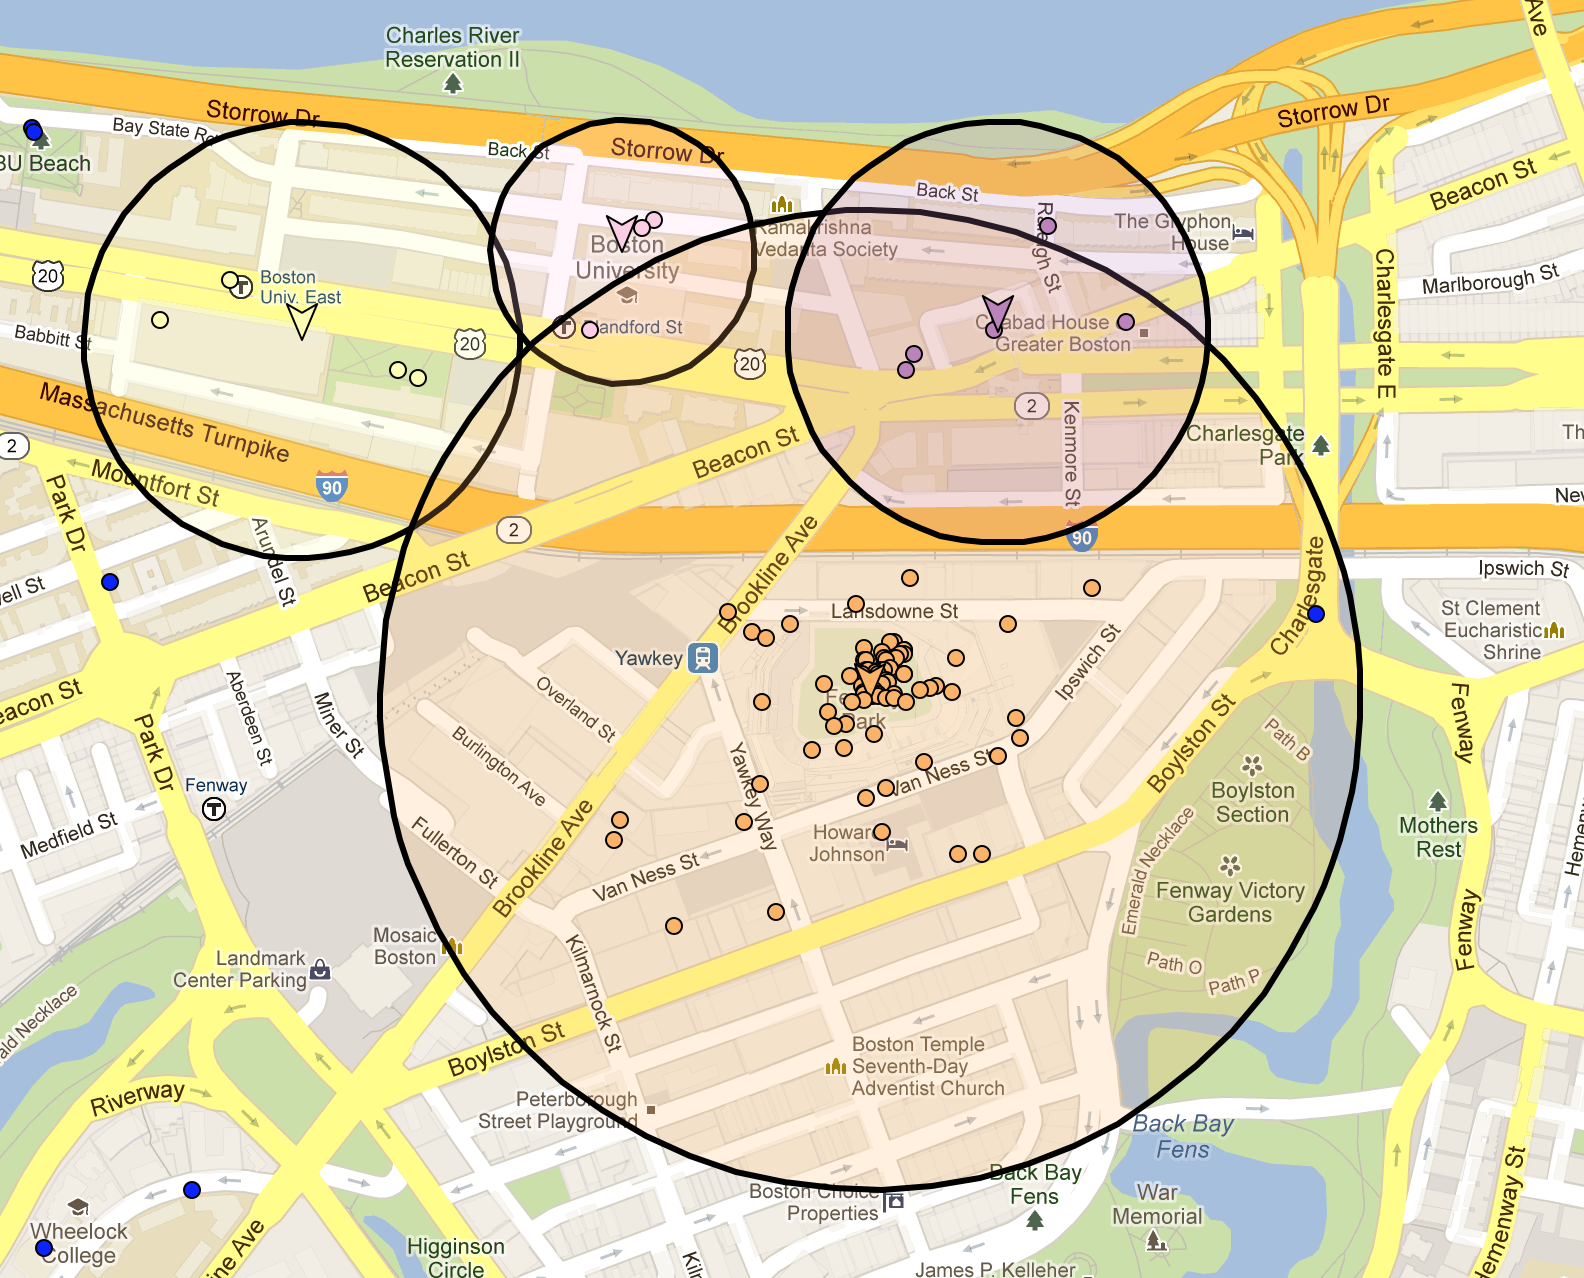
\includegraphics[width=5.5in]{fenway1.png} \\ \\
many of the clusters we found were not real events, like the one below.
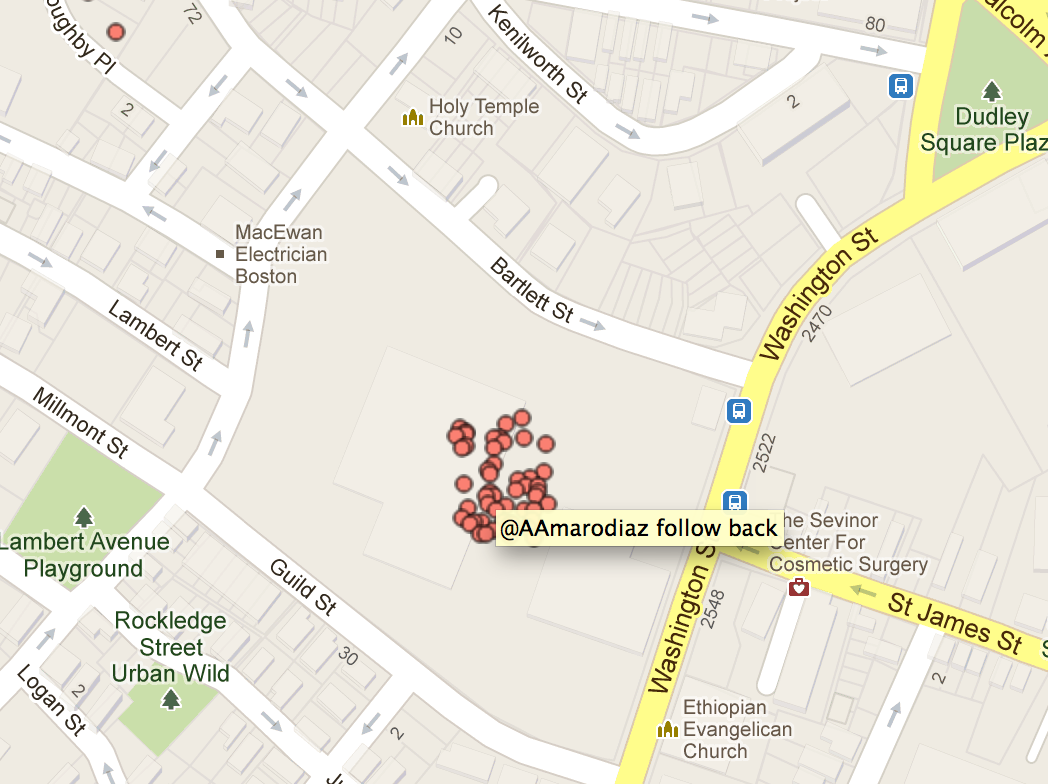
\includegraphics[width=5.5in]{lonely.png} \\ \\
One of the things we spent a lot of time on in Project III was improving this situation. With an improved clustering algorithm, that ignores clusters consisting of only a few people, and clusters tweets both temporally and geographically, the average cluster we find is of much higher quality, although the quantity of clusters we find is significantly smaller. For example, events that we recently found include a group of friends celebrating the completion of college, and several people at a hockey game (Montreal Canadiens vs. Ottowa Senators) celebrating a goal in a hockey game: \\ \\
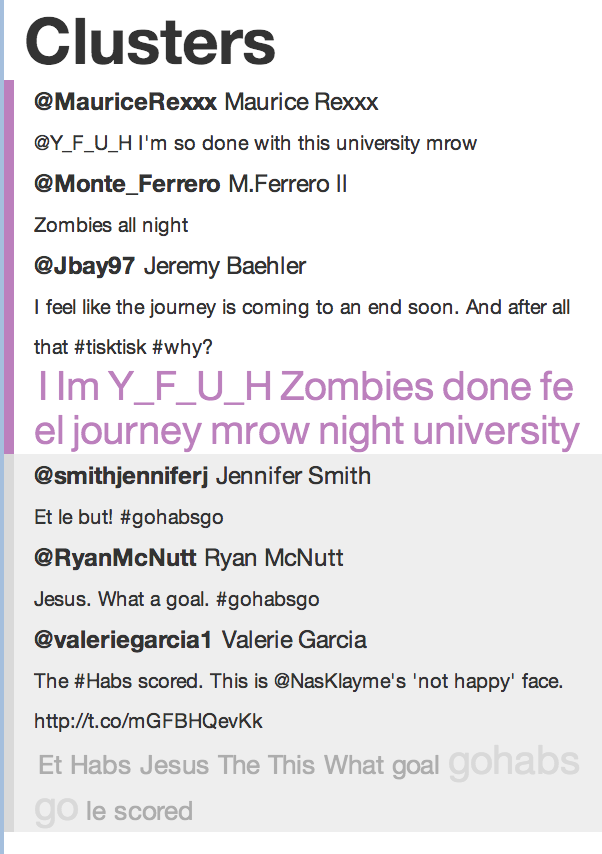
\includegraphics[width=3in]{better2.png} \\ \\
There is an important distinctions between these events and the events we found prior. These two groups of tweets are clearly very tightly related by subject matter (moreso than multiple tweets about the same baseball game), and are much smaller than the Fenway event we had identified earlier. Accordingly, our visualization is approaching the stage where it can identify both huge events like sports games and concerts, and smaller events (that may be subevents of those large events) like a goal in a sports game and a small group of people celebrating.

In addition to improving the clustering algorithm, we devoted a large amount of time in Project III to improving the way we visualized events once we found them. First, we made a word cloud for each cluster, which will hopefully allow users to understand what a cluster is about without necessarily reading through all the tweets; this visual query (identifying the content of a cluster) is extremely important to the success of the visualization. As you can see in the hockey goal event above, some of the key words highlighted by the word cloud include ``goal," ``scored," ``habs" (the nickname for the Montreal Canadiens) \footnote{http://montreal.ctvnews.ca/habs-score-four-straight-to-beat-leafs-4-1-1.1257140}, and it is pretty easy to figure out from this word cloud that this cluster represents the event that the habs scored a goal. Second, we created an additional view for our visualization, that displays the frequency of tweets over time, which allows users to brush/filter the main part of our visualization (the map) to select only tweets from a specific time period. While it is more difficult to demonstrate in one screenshot exactly what the viewer learns from such a functionality, there are several ways in which a viewer might use such a functionality. The viewer may zoom in on an event, and see the ups and downs of social data production; peaks likely indicate exciting time frames. Furthermore, the viewer can filter down to a very specific time frame and see what tweets were produced there, again possibly concluding something about what was happening in the event at that specific time frame. 

Finally, the most technically challenging aspect of our project was expanding the server-side component of our visualization. In particular, we wanted to be able to let viewers not only view live streaming twitter data, but also see pre-recorded streams of tweets that have been identified as interesting. More details about these challenges can be found in the Technical Design subsection of the Design Evolution section above.

\subsubsection{Story Telling}
While our visualization does not tell a story in the traditional sense - it is not focused on any one event or issue - we believe that it still has many story-telling aspects. In particular, we believe our visualization is a story-finding AND story-telling visualization; our visualization finds and tells a unique story to every viewer, based on their input of what (geography) they are interested in and when they are accessing our visualization.

In particular, we designed our visualization to guide users through three primary steps, which can be viewed as an opening, middle, and closing:
\begin{enumerate}
\item Our visualization opens by allowing users to select a location and a zoom on a google map, allowing them to articulate information about the types of stories they're looking for.loading tweets and identifying clusters; users watch as clusters form on the map. 
\item Next, our visualization begins loading in tweets and identifying clusters. Users can watch as clusters - which are potential stories - form on the map. 
\item Finally, our visualization closes by allowing users to learn about and explore the clusters that have been identified and the stories they represent. They see a word cloud indicating the textual content of each story, can see how the story unfolded on twitter by using the tweet frequency time chart and selecting specific time frames of tweets, and examine the individual tweets that make up the story by hovering over them on the map.
\end{enumerate}  


\section{Conclusion}
In Projects II and III, we have implemented Pheme, a real-time social data visualization. Pheme demostrates that it is possible to identify real events by examining the instantaneous social data generated by people participating in the events. Furthermore, Pheme allows users to experience and visualize events all over the world, through the social data these events generate, on their home computer, in real time.

\subsection{Future Work}
We plan on continuing to work on this project outside of CS 171. We hope to improve on Pheme in several ways in the future, including but not limited to:
\begin{enumerate}
\item More natural language processing to get even more content information out of clusters. 
\item Build in support for other languages; right now, the stopword filtration we're doing only applies to English words.
\item Detect places of interest in the world currently, and automatically drag/zoom the viewer there in the live streaming version of the visualization when they begin.
\end{enumerate} 
\end{document}
